% Figura explicativa basada en el Estado del Arte (ESQUEMA CUALITATIVO, no son datos medidos).
% Fila 1: control reactivo = solo realimentacion (umbral T/CO2, DCV) -> lineas del SotA.
%   Claves bib sugeridas: lu2022dcv (revision DCV), franco2020co2, fayos2021ventqsys (umbral CO2).
% El estado pasa a ON en t_det (ocupacion real estimada por CO2, mismo retardo); el ventilador ya
%   esta encendido desde t_in - Delta t (predictive_service._decide: PRE-COOLING mientras actual_people < 1).
% Fila 2: anticipativo = feed-forward por reserva + realimentacion CO2. En Calienfriito lo ejecuta
%   la HEURISTICA ACTIVA (predictive_service._decide usa expected_occupancy -> PRE-COOLING);
%   el modelo ML corre en sombra con la misma entrada y NO actua.
%   Claves bib sugeridas: gao2023comparative, kumkam2025comparative (control predictivo/aprendido),
%   kallio2021forecasting (pronostico de CO2/ocupacion), taheri2021learning.
% El ventilador DC no produce frio: "pre-ventilacion" renueva con aire exterior; la curva supone
%   T_ext < T_int (o mejora de sensacion termica). No se atribuye ningun resultado a nuestra heuristica.
% Caption sugerido (report-writer ajusta, con \cite verificados):
%   Control reactivo frente a anticipativo ante el ingreso de ocupantes (esquema cualitativo).
%   La estrategia reactiva, dominante en ventilacion por demanda~\cite{lu2022dcv,franco2020co2},
%   actua despues de detectar la carga; la anticipativa agrega una accion feed-forward a partir de
%   la reserva del aula, en la linea de los controladores predictivos~\cite{gao2023comparative,
%   kumkam2025comparative}. En Calienfriito esa logica la ejecuta la heuristica activa; el modelo
%   ML corre en sombra. La figura no representa mediciones.
\documentclass[tikz,border=4pt]{standalone}
\usepackage[utf8]{inputenc}
\usepackage[T1]{fontenc}
\usepackage{lmodern}
\usetikzlibrary{shapes.geometric, arrows.meta, positioning, fit, backgrounds, calc}

\definecolor{acento}{RGB}{176,30,30}   % unico acento: estrategia anticipativa (heuristica con reserva)

\tikzset{
  eje/.style     = {-{Stealth[length=2mm]}, thin},
  reac/.style    = {black, line width=1.0pt},
  antic/.style   = {acento, line width=1.5pt, dash pattern=on 5pt off 1.5pt},
  lbl/.style     = {font=\fontsize{7}{7.8}\selectfont, inner sep=1pt, align=center},
  lblb/.style    = {lbl, font=\fontsize{7.5}{8.3}\selectfont\bfseries},
  guia/.style    = {gray!60, thin, densely dotted},
  estado/.style  = {draw, thin, minimum height=4mm, inner sep=0pt, font=\fontsize{7}{7}\selectfont,
                    anchor=west},
}

% escala horizontal y instantes: inicio de pre-enfriamiento, ingreso de ocupantes, deteccion
\def\sx{0.85}
\def\tpre{2.4}
\def\tin{5.0}
\def\td{6.4}
\def\xmax{11.4}

% curvas cualitativas (Bezier explicitas, sin escalones)
\def\reactiva{(0,2.2) -- (\tin,2.2) .. controls (5.7,2.2) and (6.0,2.3) .. (6.4,2.45)
  .. controls (7.0,2.75) and (7.5,3.15) .. (8.1,3.15) .. controls (8.8,3.15) and (9.4,2.45) .. (10.2,2.2)
  .. controls (10.6,2.1) and (11.0,2.07) .. (\xmax,2.06)}
\def\anticip{(0,2.2) -- (\tpre,2.2) .. controls (3.3,2.2) and (4.1,1.85) .. (5.0,1.85)
  .. controls (5.9,1.85) and (6.8,2.3) .. (7.8,2.3) .. controls (8.6,2.3) and (9.5,2.03) .. (\xmax,2.01)}

\begin{document}
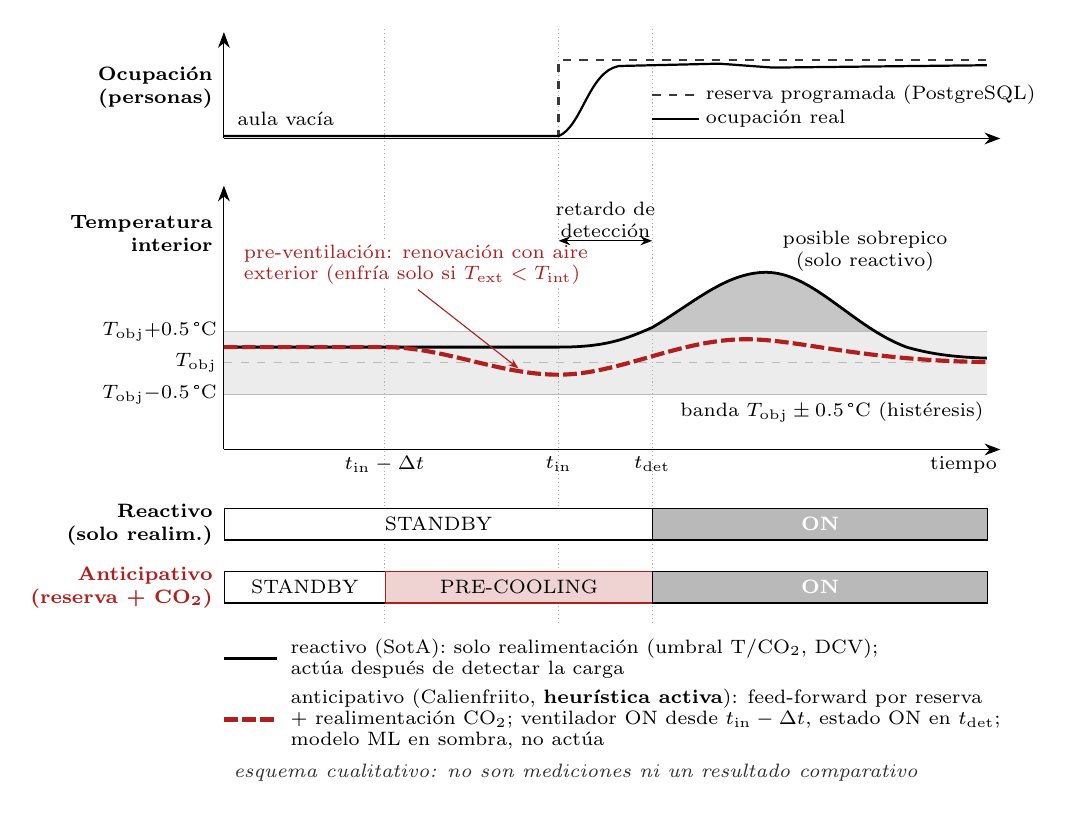
\begin{tikzpicture}[xscale=\sx]

% ======================= Panel A: ocupacion =======================
\begin{scope}[yshift=4.85cm]
  \draw[eje] (0,0) -- (\xmax+0.2,0);
  \draw[eje] (0,0) -- (0,1.35);
  \node[lblb, anchor=east, align=right] at (-0.12,0.65) {Ocupación\\(personas)};
  \draw[thick, dashed, gray!45!black] (0,0.03) -- (\tin,0.03) -- (\tin,1.0) -- (\xmax,1.0);
  \draw[thick] (0,0.03) -- (\tin,0.03) .. controls (\tin+0.35,0.15) and (\tin+0.45,0.85) .. (\tin+0.9,0.92)
               -- (7.4,0.95) -- (8.2,0.9) -- (\xmax,0.93);
  \node[lbl, anchor=south west] at (0.15,0.12) {aula vacía};
  \draw[thick, dashed, gray!45!black] (6.4,0.55) -- (7.1,0.55);
  \node[lbl, anchor=west] at (7.15,0.55) {reserva programada (PostgreSQL)};
  \draw[thick] (6.4,0.25) -- (7.1,0.25);
  \node[lbl, anchor=west] at (7.15,0.25) {ocupación real};
\end{scope}

% ======================= Panel B: temperatura =======================
\begin{scope}[on background layer]\fill[gray!15] (0,1.6) rectangle (\xmax,2.4);\end{scope}
\draw[gray!55, thin] (0,1.6) -- (\xmax,1.6) (0,2.4) -- (\xmax,2.4);
\draw[gray!55, thin, dashed] (0,2.0) -- (\xmax,2.0);
\draw[eje] (0,0.9) -- (0,4.25);
\draw[eje] (0,0.9) -- (\xmax+0.2,0.9);
\node[lblb, anchor=east, align=right] at (-0.12,3.65) {Temperatura\\interior};
\node[lbl, anchor=east] at (-0.06,2.4) {$T_{\mathrm{obj}}{+}0.5$\,°C};
\node[lbl, anchor=east] at (-0.06,2.0) {$T_{\mathrm{obj}}$};
\node[lbl, anchor=east] at (-0.06,1.6) {$T_{\mathrm{obj}}{-}0.5$\,°C};

\begin{scope}
  \clip (0,2.4) rectangle (\xmax,4.2);
  \fill[gray!45] \reactiva -- (\xmax,2.4) -- (0,2.4) -- cycle;
\end{scope}
\draw[reac]  \reactiva;
\draw[antic] \anticip;

\node[lbl, anchor=south west] at (8.3,3.12) {posible sobrepico\\(solo reactivo)};
\node[lbl, text=acento, anchor=south west, align=left, fill=white] at (0.25,2.95)
  {pre-ventilación: renovación con aire\\exterior (enfría solo si $T_{\mathrm{ext}}<T_{\mathrm{int}}$)};
\draw[acento, thin, -{Stealth[length=1.3mm]}] (2.9,2.93) -- (4.4,1.93);
\node[lbl, anchor=north east] at (\xmax,1.55) {banda $T_{\mathrm{obj}}\pm0.5$\,°C (histéresis)};

\begin{scope}[on background layer]
  \foreach \x in {\tpre,\tin,\td} \draw[guia] (\x,-1.3) -- (\x,6.25);
\end{scope}

\node[lbl, anchor=north] at (\tpre,0.85) {$t_{\mathrm{in}}-\Delta t$};
\node[lbl, anchor=north] at (\tin,0.85)  {$t_{\mathrm{in}}$};
\node[lbl, anchor=north] at (\td,0.85)   {$t_{\mathrm{det}}$};
\node[lbl, anchor=north east] at (\xmax+0.2,0.85) {tiempo};

\draw[{Stealth[length=1.5mm]}-{Stealth[length=1.5mm]}] (\tin,3.55) -- node[lbl, above] {retardo de\\detección} (\td,3.55);

% ======================= Panel C: estado del ventilador =======================
\node[lblb, anchor=east, align=right] at (-0.12,-0.05) {Reactivo\\(solo realim.)};
\node[estado, fill=white, minimum width={\td*\sx*1cm}] at (0,-0.05) {STANDBY};
\node[estado, fill=gray!55, text=white, minimum width={(\xmax-\td)*\sx*1cm}] at (\td,-0.05) {\textbf{ON}};

\node[lblb, anchor=east, align=right, text=acento] at (-0.12,-0.85) {Anticipativo\\(reserva + CO\textsubscript{2})};
\node[estado, fill=white, minimum width={\tpre*\sx*1cm}] at (0,-0.85) {STANDBY};
\node[estado, fill=acento!20, draw=acento, minimum width={(\td-\tpre)*\sx*1cm}] at (\tpre,-0.85) {PRE-COOLING};
\node[estado, fill=gray!55, text=white, minimum width={(\xmax-\td)*\sx*1cm}] at (\td,-0.85) {\textbf{ON}};

% ======================= Leyenda / aclaracion =======================
\begin{scope}[yshift=-1.75cm, font=\fontsize{7}{7.6}\selectfont]
  \draw[reac]  (0,0) -- (0.8,0);
  \node[anchor=west, align=left] at (0.85,0)
    {reactivo (SotA): solo realimentación (umbral T/CO\textsubscript{2}, DCV);\\actúa después de detectar la carga};
  \draw[antic] (0,-0.78) -- (0.8,-0.78);
  \node[anchor=west, align=left] at (0.85,-0.78)
    {anticipativo (Calienfriito, \textbf{heurística activa}): feed-forward por reserva\\+ realimentación CO\textsubscript{2}; ventilador ON desde $t_{\mathrm{in}}-\Delta t$, estado ON en $t_{\mathrm{det}}$;\\modelo ML en sombra, no actúa};
  \node[anchor=west, align=left, text=gray!35!black, font=\fontsize{7}{7.6}\selectfont\itshape] at (0,-1.45)
    {esquema cualitativo: no son mediciones ni un resultado comparativo};
\end{scope}


\end{tikzpicture}
\end{document}
